\subsection{Neuroevolution of augmenting topologies}
Neuroevolution uses evolutionary algorithms to optimise ANNs \cite{neuroevolution_review}.
One such algorithm is Neuroevolution of Augmenting Topologies (NEAT), which evolves the topology and weights of ANNs
using a genetic algorithm \cite{neat_main, neat_short, neat_phd}.

NEAT uses a direct encoding; genomes contain connection- and node genes which specify the corresponding
network (see Figure \ref{mapping}). Each connection gene is identified by a number and
references the two node genes it spans. The node gene is also identified by a number.

\setlength{\arrayrulewidth}{1mm}
\setlength{\tabcolsep}{5pt}
\renewcommand{\arraystretch}{1}

%\newcolumntype{s}{>{\columncolor[HTML]{AAACED}} p{0.5cm}}

\arrayrulecolor[HTML]{DB5800}

\begin{tabular}{ |p{0.5cm}|p{0.5cm}|p{0.7cm}|p{1.5cm}|p{1.5cm}|  }
    \hline
    \multicolumn{5}{|c|}{Connection genes} \\

    \hline
    Id & In & Out & Weight & Enabled \\

    \hline

\end{tabular}

The initial population of genomes encode structurally identical and fully connected networks without any hidden nodes.
New structures emerge through structural mutations which can add genes for new connections and nodes to the genomes.
Nodes are added by splitting an existing connection, which is then disabled and two new connection genes are added along
with the new node gene (see Figure \ref{node_mutation}).

\begin{figure}[htb]
    \begin{mdframed}
        \begin{subfigure}[b]{0.45\textwidth}
            \centering
            \resizebox{1\textwidth}{!}{\setlength{\arrayrulewidth}{0.01mm}
\setlength{\tabcolsep}{5pt}
\renewcommand{\arraystretch}{1}

\arrayrulecolor[HTML]{000000}

\vspace{0.2cm}
\begin{tabular}{ |p{0.5cm}|p{1.8cm}|  }
    \hline
    \rowcolor{lightgray} \multicolumn{2}{|c|}{Node genes} \\
    \hline
    Id & Type \\
    \hline
    1 & \cellcolor{green!50} INPUT \\
    \hline
    2 & \cellcolor{green!50} INPUT \\
    \hline
    3 & \cellcolor{red!50} OUTPUT \\
    \hline
    4 & \cellcolor{blue!50} HIDDEN \\
    \hline
\end{tabular}

\begin{tabular}{ |p{0.5cm}|p{0.5cm}|p{0.7cm}|p{1.2cm}|p{1.4cm}|  }
    \hline
    \rowcolor{lightgray} \multicolumn{5}{|c|}{Connection genes} \\
    \hline
    Id & In & Out & Weight & Enabled \\
    \hline
    1 & \cellcolor{green!50} 1 & \cellcolor{red!50} 3 & 0.3 & True \\
    2 & \cellcolor{green!50} 2 & \cellcolor{red!50} 3 & 0.5 & False \\
    3 & \cellcolor{green!50} 2 & \cellcolor{blue!50} 4 & 1 & True \\
    4 & \cellcolor{blue!50} 4 & \cellcolor{red!50} 2 & 0.5 & True \\
    \hline
\end{tabular}
}
            \caption{Genotype.}
            \label{node_genotype}
        \end{subfigure}
        \begin{subfigure}[b]{0.45\textwidth}
            \centering
            \resizebox{0.65\textwidth}{!}{\def\layersep{2.5cm}

\begin{tikzpicture}[shorten >=1pt,->,draw=black!50, node distance=\layersep]
    \tikzstyle{every pin edge}=[<-,shorten <=1pt]
    \tikzstyle{neuron}=[circle,fill=black!25,minimum size=17pt,inner sep=0pt]
    \tikzstyle{input neuron}=[neuron, fill=green!50];
    \tikzstyle{output neuron}=[neuron, fill=red!50];
    \tikzstyle{hidden neuron}=[neuron, fill=blue!50];

    % Draw the input nodes.
    \foreach \name / \y in {1,...,2}
        \node[input neuron] (I-\name) at (0,-\y) {\y};

    %Draw the hidden node.
    \node[hidden neuron, right of=I-2] (H-1) {4};

    % Draw the output node.
    \node[output neuron, right of=H-2] (O-1) {3};

    % Connect input 1 with output node.
    \path (I-1) edge (O-1);
    \path (I-2) edge (H-1);
    \path (H-1) edge (O-1);

    \draw (I-1) -- (O-1) node [midway, fill=white] {1};
    \draw (I-2) -- (H-1) node [midway, fill=white] {3};
    \draw (H-1) -- (O-1) node [midway, fill=white] {4};

\end{tikzpicture}}
            \caption{Phenotype.}
            \label{node_phenotype}
        \end{subfigure}
    \end{mdframed}
    \caption{Example of a node mutation.}
    \label{node_mutation}
\end{figure}


Mutations can also add new connections, which span any two previously unconnected nodes in the genome (see Figure \ref{link_mutation}).
Connections can be of three types, depending on their output node. Loops are connections that start and end on the same node. Recurrent
connections go backwards in the network to a node closer to an input node. Finally, forward connections end on a node closer to an output
node. The first two types of connections can provide a form of short term memory by repeating signals from a previous time step.

\begin{figure}[htb]
    \begin{mdframed}
        \begin{subfigure}[b]{0.45\textwidth}
            \centering
            \resizebox{1\textwidth}{!}{\setlength{\arrayrulewidth}{0.01mm}
\setlength{\tabcolsep}{5pt}
\renewcommand{\arraystretch}{1}

\arrayrulecolor[HTML]{000000}

\vspace{0.2cm}
\begin{tabular}{ |p{0.5cm}|p{1.8cm}|  }
    \hline
    \rowcolor{lightgray} \multicolumn{2}{|c|}{Node genes} \\
    \hline
    ID & Type \\
    \hline
    1 & \cellcolor{green!50} INPUT \\
    \hline
    2 & \cellcolor{green!50} INPUT \\
    \hline
    3 & \cellcolor{red!50} OUTPUT \\
    \hline
    4 & \cellcolor{blue!50} HIDDEN \\
    \hline
\end{tabular}

\begin{tabular}{ |p{0.5cm}|p{0.5cm}|p{0.7cm}|p{1.2cm}|p{1.4cm}|  }
    \hline
    \rowcolor{lightgray} \multicolumn{5}{|c|}{Connection genes} \\
    \hline
    ID & In & Out & Weight & Enabled \\
    \hline
    1 & \cellcolor{green!50} 1 & \cellcolor{red!50} 3 & 0.3 & True \\
    2 & \cellcolor{green!50} 2 & \cellcolor{red!50} 3 & 0.5 & False \\
    3 & \cellcolor{green!50} 2 & \cellcolor{blue!50} 4 & 1 & True \\
    4 & \cellcolor{blue!50} 4 & \cellcolor{red!50} 2 & 0.5 & True \\
    5 & \cellcolor{green!50} 1 & \cellcolor{blue!50} 4 & 0.4 & True \\
    \hline
\end{tabular}
}
            \caption{Genotype.}
            \label{link_genotype}
        \end{subfigure}
        \begin{subfigure}[b]{0.45\textwidth}
            \centering
            \resizebox{0.65\textwidth}{!}{\def\layersep{2.5cm}

\begin{tikzpicture}[shorten >=1pt,->,draw=black!50, node distance=\layersep]
    \tikzstyle{every pin edge}=[<-,shorten <=1pt]
    \tikzstyle{neuron}=[circle,fill=black!25,minimum size=17pt,inner sep=0pt]
    \tikzstyle{input neuron}=[neuron, fill=green!50];
    \tikzstyle{output neuron}=[neuron, fill=red!50];
    \tikzstyle{hidden neuron}=[neuron, fill=blue!50];

    % Draw the input nodes.
    \foreach \name / \y in {1,...,2}
        \node[input neuron] (I-\name) at (0,-\y) {\y};

    %Draw the hidden node.
    \node[hidden neuron, right of=I-2] (H-1) {4};

    % Draw the output node.
    \node[output neuron, right of=H-2] (O-1) {3};


    \draw (I-1) -- (O-1) node [midway, fill=white] {1};
    \draw (I-2) -- (H-1) node [midway, fill=white] {3};
    \draw (H-1) -- (O-1) node [midway, fill=white] {4};
    \draw (I-1) -- (H-1) node [midway, fill=white] {5};
\end{tikzpicture}}
            \caption{Phenotype.}
            \label{link_phenotype}
        \end{subfigure}
    \end{mdframed}
    \caption{ (a) The resulting genotype after a link mutation of the genotype from \ref{node_mutation}(a). (b) The
    corresponding network phenotype with a new forward link between nodes 1 and 4.}
    \label{link_mutation}
\end{figure}


The ID attribute of the genes, referred to as an innovation number, serves to uniquely identify each mutation that has occurred.
Each time a new link or node is added, a database containing all previous mutations and their IDs is referenced. That way,
identical links and nodes are labelled with the same ID.

NEAT protects new structures by placing similar networks in the population into species.
Competition mainly occurs within the species, ensuring newly created structures are not prematurely deleted.
Since each gene is labelled with an ID, computing a measure of structural similarity is as simple as
comparing IDs in the genomes.

The IDs are also used during crossover to create meaningful offspring from networks with different structure.
They indicate the origin of each gene, making it possible to align homologous genes in the genomes. Genes
that are not present in both genomes are only inherited from the more fit parent.

\begin{tikzpicture}

    \begin{scope}
        
% Population
\node [box] (population) {};
\node [anchor=north] at (population.north) {Population};

\node (line1) [anchor=south west] at (population.south west) {$\coloredrule{10mm}{1mm}{green!50}$};
\node (line2) [anchor=south west] at (line1.south east) {$\coloredrule{10mm}{1mm}{red!25}$};
\node (line3) [anchor=south west] at (line2.south east) {$\coloredrule{10mm}{1mm}{blue!50}$};
\node (line4) [anchor=south west] at (line1.north west) {$\coloredrule{10mm}{1mm}{red!50}$};
\node (line5) [anchor=south west] at (line2.north west) {$\coloredrule{10mm}{1mm}{lime!50}$};
\node (line6) [anchor=south west] at (line3.north west) {$\coloredrule{10mm}{1mm}{blue!75}$};
\node (line7) [anchor=south west] at (line4.north west) {$\coloredrule{10mm}{1mm}{blue!25}$};
\node (line8) [anchor=south west] at (line5.north west) {$\coloredrule{10mm}{1mm}{red!75}$};
\node (line9) [anchor=south west] at (line6.north west) {$\coloredrule{10mm}{1mm}{teal!50}$};

    \end{scope}

    \begin{scope}[xshift=4.5cm]
        
\begin{tikzpicture}
    \tikzstyle{box} = [rectangle, rounded corners, minimum width=4cm, minimum height=1.8cm,text centered, draw=black, fill=gray!10]

    % Phenotypes
    \node [box] (phenotypes) {};
    \node [anchor=north] at (phenotypes.north) {phenotypes};
    \node (phenotype1) [anchor=south west] at (phenotypes.south west) {\resizebox{0.05\textwidth}{!}{\def\layersep{2.5cm}

\begin{tikzpicture}[shorten >=1pt,->,draw=black!50, node distance=\layersep]
    \tikzstyle{every pin edge}=[<-,shorten <=1pt]
    \tikzstyle{neuron}=[circle,fill=black!25,minimum size=17pt,inner sep=0pt]
    \tikzstyle{input neuron}=[neuron, fill=green!50];
    \tikzstyle{output neuron}=[neuron, fill=red!50];

    % Draw the input nodes.
    \foreach \name / \y in {1,...,2}
        \node[input neuron] (I-\name) at (0,-\y) {};

    % Draw the output node.
    \node[output neuron, right of=H-2] (O-1) {};

    % Connect inputs with output node.
    \draw (I-1) -- (O-1);
    \draw (I-2) -- (O-1);
\end{tikzpicture}}};
    %\node (phenotype2) [anchor=south west] at (phenotype1.south west) {\resizebox{0.05\textwidth}{!}{\def\layersep{2.5cm}

\begin{tikzpicture}[shorten >=1pt,->,draw=black!50, node distance=\layersep]
    \tikzstyle{every pin edge}=[<-,shorten <=1pt]
    \tikzstyle{neuron}=[circle,fill=black!25,minimum size=17pt,inner sep=0pt]
    \tikzstyle{input neuron}=[neuron, fill=green!50];
    \tikzstyle{output neuron}=[neuron, fill=red!50];

    % Draw the input nodes.
    \foreach \name / \y in {1,...,2}
        \node[input neuron] (I-\name) at (0,-\y) {};

    % Draw the output node.
    \node[output neuron, right of=H-2] (O-1) {};

    % Connect inputs with output node.
    \draw (I-1) -- (O-1);
    \draw (I-2) -- (O-1);
\end{tikzpicture}}};
    %\node (phenotype3) [anchor=south west] at (phenotype2.south west) {\resizebox{0.05\textwidth}{!}{\def\layersep{2.5cm}

\begin{tikzpicture}[shorten >=1pt,->,draw=black!50, node distance=\layersep]
    \tikzstyle{every pin edge}=[<-,shorten <=1pt]
    \tikzstyle{neuron}=[circle,fill=black!25,minimum size=17pt,inner sep=0pt]
    \tikzstyle{input neuron}=[neuron, fill=green!50];
    \tikzstyle{output neuron}=[neuron, fill=red!50];

    % Draw the input nodes.
    \foreach \name / \y in {1,...,2}
        \node[input neuron] (I-\name) at (0,-\y) {};

    % Draw the output node.
    \node[output neuron, right of=H-2] (O-1) {};

    % Connect inputs with output node.
    \draw (I-1) -- (O-1);
    \draw (I-2) -- (O-1);
\end{tikzpicture}}};
\end{tikzpicture}
    \end{scope}

    \begin{scope}[xshift=9cm]
        
\node [box] (evaluation) {};
\node [anchor=north] at (evaluation.north) {Evaluation};


    \end{scope}

    \begin{scope}[xshift=9cm, yshift=-3cm]
        
\node [box] (speciate) {};
\node [anchor=north] at (speciate.north) {Speciation};

\node (line1) [anchor=south west] at (speciate.south west) {$\coloredrule{10mm}{1mm}{OliveGreen}$};
\node (line2) [anchor=south west] at (line1.south east) {$\coloredrule{10mm}{1mm}{RubineRed}$};
\node (line3) [anchor=south west] at (line2.south east) {$\coloredrule{10mm}{1mm}{blue}$};
\node (line4) [anchor=south west] at (line1.north west) {$\coloredrule{10mm}{1mm}{green}$};
\node (line5) [anchor=south west] at (line2.north west) {$\coloredrule{10mm}{1mm}{red}$};
\node (line6) [anchor=south west] at (line3.north west) {$\coloredrule{10mm}{1mm}{Periwinkle}$};
\node (line7) [anchor=south west] at (line4.north west) {$\coloredrule{10mm}{1mm}{SeaGreen}$};
\node (line8) [anchor=south west] at (line5.north west) {$\coloredrule{10mm}{1mm}{Salmon}$};
\node (line9) [anchor=south west] at (line6.north west) {$\coloredrule{10mm}{1mm}{Cyan}$};


    \end{scope}

    \begin{scope}[xshift=9cm, yshift=-6cm]
        
\node [box] (selection) {};
\node [anchor=north] at (selection.north) {Selection};

\node (line1) [anchor=south west] at (selection.south west) {$\coloredrule{10mm}{1mm}{OliveGreen}$};
\node (line2) [anchor=south west] at (line1.south east) {$\coloredrule{10mm}{1mm}{Red}$};
\node (line3) [anchor=south west] at (line2.south east) {$\coloredrule{10mm}{1mm}{blue}$};
\node (line4) [anchor=south west] at (line1.north west) {$\coloredrule{10mm}{1mm}{green}$};
\node (line5) [anchor=south west] at (line2.north west) {$\coloredrule{10mm}{1mm}{Salmon}$};
\node (line6) [anchor=south west] at (line3.north west) {$\coloredrule{10mm}{1mm}{Periwinkle}$};

    \end{scope}

    \begin{scope}[xshift=4.5cm, yshift=-6cm]
        

\node [box] (reproduction) {};
\node [anchor=north] at (reproduction.north) {Reproduction};

\node (line1) [anchor=south west] at (reproduction.south west) {$\coloredrule{10mm}{1mm}{OliveGreen, green}$};
\node (line2) [anchor=south west] at (line1.south east) {$\coloredrule{10mm}{1mm}{red, Salmon}$};
\node (line3) [anchor=south west] at (line2.south east) {$\coloredrule{10mm}{1mm}{blue, Periwinkle}$};
\node (line4) [anchor=south west] at (line1.north west) {$\coloredrule{10mm}{1mm}{green, OliveGreen}$};
\node (line5) [anchor=south west] at (line2.north west) {$\coloredrule{10mm}{1mm}{Salmon, red}$};
\node (line6) [anchor=south west] at (line3.north west) {$\coloredrule{10mm}{1mm}{Periwinkle, blue}$};
\node (line7) [anchor=south west] at (line4.north west) {$\coloredrule{10mm}{1mm}{green}$};
\node (line8) [anchor=south west] at (line5.north west) {$\coloredrule{10mm}{1mm}{red}$};
\node (line9) [anchor=south west] at (line6.north west) {$\coloredrule{10mm}{1mm}{blue}$};
    \end{scope}

    \begin{scope}[xshift=0cm, yshift=-6cm]
        
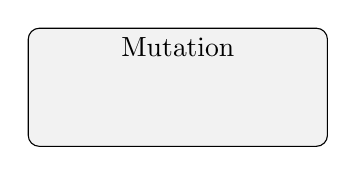
\begin{tikzpicture}
    \tikzstyle{box} = [rectangle, rounded corners, minimum width=3.8cm, minimum height=1.5cm,text centered, draw=black, fill=gray!10]

    \node [box] (mutation) {};
    \node [anchor=north] at (mutation.north) {Mutation};

    % TODO: slightly shift the color of the offspring.

  \end{tikzpicture}
    \end{scope}

\end{tikzpicture}

